\PassOptionsToPackage{table}{xcolor}
\documentclass[aspectratio=169]{beamer}\usepackage[utf8]{inputenc}
\usepackage{lmodern}
\usepackage[english]{babel}
\usepackage{color}
\usepackage{amsmath,mathtools}
\usepackage{booktabs}
\usepackage{mathptmx}
\usepackage[11pt]{moresize}
\usepackage{hyperref}
\usepackage{commath}
\usepackage{bm}
\usepackage{subfigure}
\usepackage{siunitx}

\setbeamertemplate{navigation symbols}{}
\setbeamersize{text margin left=5mm,text margin right=5mm}
\setbeamertemplate{caption}[numbered]
\addtobeamertemplate{navigation symbols}{}{
\usebeamerfont{footline}
\usebeamercolor[fg]{footline}
\hspace{1em}
\insertframenumber/\inserttotalframenumber}

\newcommand{\R}{\mathbb{R}}
\newcommand{\E}{\mathbb{E}}
\newcommand{\N}{\mathbb{N}}
\newcommand{\Z}{\mathbb{Z}}
\newcommand{\V}{\mathbb{V}}
\newcommand{\Q}{\mathbb{Q}}
\newcommand{\K}{\mathbb{K}}
\newcommand{\C}{\mathbb{C}}
\newcommand{\T}{\mathbb{T}}
\newcommand{\I}{\mathbb{I}}
\DeclareMathOperator{\sign}{sign}

\title{Error SDE ($Z_t$) moments}
\subtitle{Renzo Miguel Caballero Rosas}

\begin{document}

\begin{frame}
\titlepage
\end{frame}


\setbeamercolor{background canvas}{bg=white!10}
\begin{frame}\frametitle{Data histograms:}

\begin{figure}[ht!]
\centering
\includegraphics[width=0.3\textwidth]{../../MATLAB_Files/Results/histograms/others/forecast_transitions.eps}\quad
\includegraphics[width=0.3\textwidth]{../../MATLAB_Files/Results/histograms/others/error_measurement.eps}\quad
\includegraphics[width=0.3\textwidth]{../../MATLAB_Files/Results/histograms/others/error_and_forecast.eps}
\end{figure}
From here we can see that the errors are approximately in the interval $[-0.3,0.3]$, and the forecast transitions in the interval $[-0.03,0.03]$.\\
Then, we want to ensure that the moments are well approximated in the rectangle $[-0.3,0.3]\times[-0.03,0.03]$ (for $V\times\Delta p$).

\end{frame}


\setbeamercolor{background canvas}{bg=white!10}
\begin{frame}\frametitle{Approximated moments for $Z_t$:}

\begin{figure}[ht!]
\centering
\includegraphics[width=0.3\textwidth]{../../MATLAB_Files/Results/moments/lamperti/errors/fm_ODE_1.eps}\quad
\includegraphics[width=0.3\textwidth]{../../MATLAB_Files/Results/moments/lamperti/errors/fm_MC_1.eps}\quad
\includegraphics[width=0.3\textwidth]{../../MATLAB_Files/Results/moments/lamperti/errors/fm_1.eps}\quad
\includegraphics[width=0.3\textwidth]{../../MATLAB_Files/Results/moments/lamperti/errors/sm_ODE_1.eps}\quad
\includegraphics[width=0.3\textwidth]{../../MATLAB_Files/Results/moments/lamperti/errors/sm_MC_1.eps}\quad
\includegraphics[width=0.3\textwidth]{../../MATLAB_Files/Results/moments/lamperti/errors/sm_1.eps}
\end{figure}

\end{frame}


\setbeamercolor{background canvas}{bg=white!10}
\begin{frame}\frametitle{Approximated moments for $Z_t$:}

\begin{figure}[ht!]
\centering
\includegraphics[width=0.3\textwidth]{../../MATLAB_Files/Results/moments/lamperti/errors/fm_ODE_2.eps}\quad
\includegraphics[width=0.3\textwidth]{../../MATLAB_Files/Results/moments/lamperti/errors/fm_MC_2.eps}\quad
\includegraphics[width=0.3\textwidth]{../../MATLAB_Files/Results/moments/lamperti/errors/fm_2.eps}\quad
\includegraphics[width=0.3\textwidth]{../../MATLAB_Files/Results/moments/lamperti/errors/sm_ODE_2.eps}\quad
\includegraphics[width=0.3\textwidth]{../../MATLAB_Files/Results/moments/lamperti/errors/sm_MC_2.eps}\quad
\includegraphics[width=0.3\textwidth]{../../MATLAB_Files/Results/moments/lamperti/errors/sm_2.eps}
\end{figure}

\end{frame}


\setbeamercolor{background canvas}{bg=white!10}
\begin{frame}\frametitle{Approximated moments for $Z_t$:}

\begin{figure}[ht!]
\centering
\includegraphics[width=0.3\textwidth]{../../MATLAB_Files/Results/moments/lamperti/errors/fm_ODE_3.eps}\quad
\includegraphics[width=0.3\textwidth]{../../MATLAB_Files/Results/moments/lamperti/errors/fm_MC_3.eps}\quad
\includegraphics[width=0.3\textwidth]{../../MATLAB_Files/Results/moments/lamperti/errors/fm_3.eps}\quad
\includegraphics[width=0.3\textwidth]{../../MATLAB_Files/Results/moments/lamperti/errors/sm_ODE_3.eps}\quad
\includegraphics[width=0.3\textwidth]{../../MATLAB_Files/Results/moments/lamperti/errors/sm_MC_3.eps}\quad
\includegraphics[width=0.3\textwidth]{../../MATLAB_Files/Results/moments/lamperti/errors/sm_3.eps}
\end{figure}

\end{frame}


\setbeamercolor{background canvas}{bg=white!10}
\begin{frame}\frametitle{Approximated moments for $Z_t$:}

\begin{figure}[ht!]
\centering
\includegraphics[width=0.3\textwidth]{../../MATLAB_Files/Results/moments/lamperti/errors/fm_ODE_4.eps}\quad
\includegraphics[width=0.3\textwidth]{../../MATLAB_Files/Results/moments/lamperti/errors/fm_MC_4.eps}\quad
\includegraphics[width=0.3\textwidth]{../../MATLAB_Files/Results/moments/lamperti/errors/fm_4.eps}\quad
\includegraphics[width=0.3\textwidth]{../../MATLAB_Files/Results/moments/lamperti/errors/sm_ODE_4.eps}\quad
\includegraphics[width=0.3\textwidth]{../../MATLAB_Files/Results/moments/lamperti/errors/sm_MC_4.eps}\quad
\includegraphics[width=0.3\textwidth]{../../MATLAB_Files/Results/moments/lamperti/errors/sm_4.eps}
\end{figure}

\end{frame}


\setbeamercolor{background canvas}{bg=white!10}
\begin{frame}\frametitle{Approximated moments for $Z_t$:}

\begin{figure}[ht!]
\centering
\includegraphics[width=0.3\textwidth]{../../MATLAB_Files/Results/moments/lamperti/errors/fm_ODE_5.eps}\quad
\includegraphics[width=0.3\textwidth]{../../MATLAB_Files/Results/moments/lamperti/errors/fm_MC_5.eps}\quad
\includegraphics[width=0.3\textwidth]{../../MATLAB_Files/Results/moments/lamperti/errors/fm_5.eps}\quad
\includegraphics[width=0.3\textwidth]{../../MATLAB_Files/Results/moments/lamperti/errors/sm_ODE_5.eps}\quad
\includegraphics[width=0.3\textwidth]{../../MATLAB_Files/Results/moments/lamperti/errors/sm_MC_5.eps}\quad
\includegraphics[width=0.3\textwidth]{../../MATLAB_Files/Results/moments/lamperti/errors/sm_5.eps}
\end{figure}

\end{frame}


\setbeamercolor{background canvas}{bg=white!10}
\begin{frame}\frametitle{Approximated moments for $Z_t$:}

\begin{figure}[ht!]
\centering
\includegraphics[width=0.3\textwidth]{../../MATLAB_Files/Results/moments/lamperti/errors/fm_ODE_6.eps}\quad
\includegraphics[width=0.3\textwidth]{../../MATLAB_Files/Results/moments/lamperti/errors/fm_MC_6.eps}\quad
\includegraphics[width=0.3\textwidth]{../../MATLAB_Files/Results/moments/lamperti/errors/fm_6.eps}\quad
\includegraphics[width=0.3\textwidth]{../../MATLAB_Files/Results/moments/lamperti/errors/sm_ODE_6.eps}\quad
\includegraphics[width=0.3\textwidth]{../../MATLAB_Files/Results/moments/lamperti/errors/sm_MC_6.eps}\quad
\includegraphics[width=0.3\textwidth]{../../MATLAB_Files/Results/moments/lamperti/errors/sm_6.eps}
\end{figure}

\end{frame}


\setbeamercolor{background canvas}{bg=white!10}
\begin{frame}\frametitle{Approximated moments for $Z_t$:}

\begin{figure}[ht!]
\centering
\includegraphics[width=0.3\textwidth]{../../MATLAB_Files/Results/moments/lamperti/errors/fm_ODE_7.eps}\quad
\includegraphics[width=0.3\textwidth]{../../MATLAB_Files/Results/moments/lamperti/errors/fm_MC_7.eps}\quad
\includegraphics[width=0.3\textwidth]{../../MATLAB_Files/Results/moments/lamperti/errors/fm_7.eps}\quad
\includegraphics[width=0.3\textwidth]{../../MATLAB_Files/Results/moments/lamperti/errors/sm_ODE_7.eps}\quad
\includegraphics[width=0.3\textwidth]{../../MATLAB_Files/Results/moments/lamperti/errors/sm_MC_7.eps}\quad
\includegraphics[width=0.3\textwidth]{../../MATLAB_Files/Results/moments/lamperti/errors/sm_7.eps}
\end{figure}

\end{frame}


\setbeamercolor{background canvas}{bg=white!10}
\begin{frame}\frametitle{Approximated moments for $Z_t$:}

\begin{figure}[ht!]
\centering
\includegraphics[width=0.5\textwidth]{../../MATLAB_Files/Results/moments/lamperti/7.eps}
\end{figure}

\end{frame}

\end{document}